% 2000 年全国新课程卷文科第 18 题乙：平行六面体 ABCD-A_1B_1C_1D_1
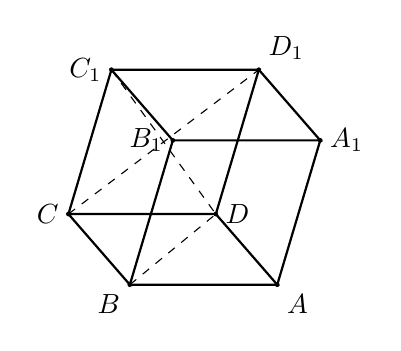
\begin{tikzpicture}[>=stealth, scale=0.78]
  \coordinate (A) at (3.4,0);
  \coordinate (B) at (1.0,0);
  \coordinate (C) at (0,1.15);
  \coordinate (D) at (2.4,1.15);
  \coordinate (A1) at (4.1,2.35);
  \coordinate (B1) at (1.7,2.35);
  \coordinate (C1) at (0.7,3.5);
  \coordinate (D1) at (3.1,3.5);

  \draw[thick] (A)--(B)--(C)--(D)--cycle;
  \draw[thick] (A1)--(B1)--(C1)--(D1)--cycle;
  \draw[thick] (A)--(A1) (B)--(B1) (C)--(C1) (D)--(D1);
  \draw[dashed] (C1)--(D) (B)--(D) (C)--(D1);

  \fill (A) circle (1.1pt) node[below right] {$A$};
  \fill (B) circle (1.1pt) node[below left] {$B$};
  \fill (C) circle (1.1pt) node[left] {$C$};
  \fill (D) circle (1.1pt) node[right] {$D$};
  \fill (A1) circle (1.1pt) node[right] {$A_1$};
  \fill (B1) circle (1.1pt) node[left] {$B_1$};
  \fill (C1) circle (1.1pt) node[left] {$C_1$};
  \fill (D1) circle (1.1pt) node[above right] {$D_1$};
\end{tikzpicture}
